\chapter{基于国产AI处理器的Top-k算法测试验证}

本章首先介绍了Topk-k算子测试用到的实验环境,同时也描述了整个算子测试的流程。
接着自行编写脚本生成大量的测试用例,用于测试自实现 Top-k 算子的准确度是否满足要求,
以确认功能是否正确。
然后测试了不同输入规模下,Topk 算子相对于全排序Top-k算子 和 Nvidia芯片上Top-k算子的性能表现情况。
最后将自实现
 Top-k 算子集成在Pytorch深度学习框架中,对目前比较流行的模型进行训练,
 并通过检测结果验证了Top-k 算子的可用性。

\section{实验环境与测试流程}
\subsection{实验环境}

测试的环境配置如表~\ref{tab:peizhi}所示。
\begin{table}[h]
    \centering
    \caption{硬件环境配置}
    \begin{tabular}{|l|l|}
    \hline
    类型 & 配置信息 \\
    \hline
    AI处理器 & DLP-M处理器 \\
    \hline
    CPU & Intel Xeon Silver 4114 \\
    \hline
    Nvidia GPU & A100-40G \\
    \hline
    操作系统 & CentOS - 7 \\
    \hline
    开发语言 & BC 4.7.0, C++11, Python 2.7.5 \\
    \hline
    编译器 & CC 4.7.1, gcc 4.8.5 \\
    \hline
    \end{tabular}
    \label{tab:peizhi}
    \end{table}
    
    本次实验以 CPU+国产AI 处理器(以下简称 MLU)异构编程模式进行,用到了BC、C++ 以及 Python 
    三种编程语言。BC 编程语言用于实现 MLU 端的 Top-k 算法计算过程;
    C++ 编程语言则用于实现 CPU 端的数据准备;
    Python 编程语言用于 编写测例用例生成脚本。
    CC(Compiler Collection,BC 语言编译器)是基于 Clang和 LLVM 开发的 BC 编译器主驱动程序
    ,负责将 BC 源码文件编译为 MLISA 汇编文件。
    

\subsection{测试流程}
\begin{enumerate}
    \item 通过 RT 接口初始化设备,RT 包含设备管理、内存管理、任务队列管理、 设备端程序执行、通知管理等功能,使用 BC 编写的程序需要借助于 RT 提供的 接口才能运行在 MLU 设备上。
    \item 初始化 Top-k 描述符,并为保存 Top-k 参数内容的结构体创建一个句柄。 同时计算出当前输入参数下计算得到的 Top-k 特征向量需要占用的内存空间大 小, 并分配对应的内存空间。
    \item 准备输入数据,调用 RT 接口分配设备内存,并将输入数据拷贝到设备 内存中。
    \item MLU 端调用自实现的 Top 算子,得到 Top-看 特征向量。CPU 端调用 RT接口等待任务队列执行完成。
    
    \item 调用RT接口将Top-k算子的计算结果复制到主机侧。
    \item 主机侧调用Top-k的串行实现,得到比对的计算结果。
    \item 将设备端的计算结果与主机端的计算结果进行比较。
    \item 调用RT接口,释放主机端和设备端的内存以及任务队列等资源。
    
\end{enumerate}
整个计算流程如图~\ref{fig:test}所示:

\begin{figure}[ht]
    \centering
    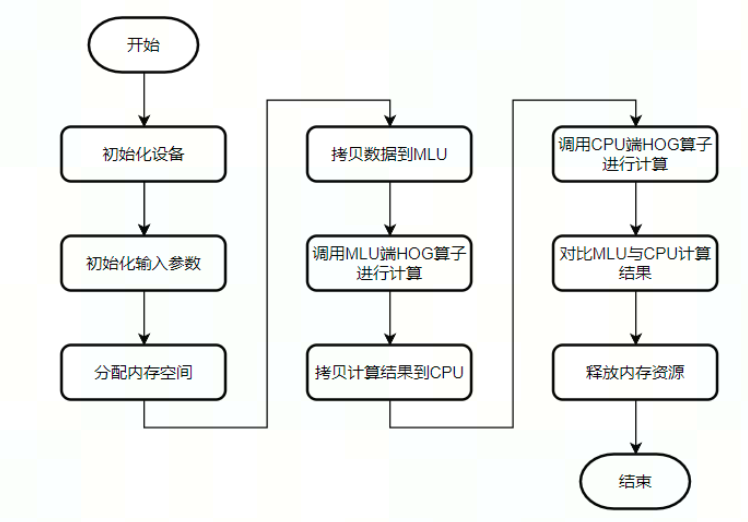
\includegraphics[width=1.0\textwidth]{test.png}
    \caption{RadixSelect测试流程图}
    \label{fig:test}
    % \note{注:图注的内容不宜放到图题中。}
\end{figure}


\section{Top-k算子功能测试}
在完成深度学习处理器的Top - K算子实现后,便可以开展算子的功能性与性能验证工作。
首先是功能验证,其主要内容如下:
\begin{enumerate}
\item 对不同维度(dim)下Top-k查询结果的正确性进行验证。
\item 针对不同k值下的查询结果正确性进行验证。
\item 检验经largest排序后的数据返回是否正确。
\end{enumerate}

在进行Top-k正确性验证时,将计算结果与CPU计算结果进行对比,
误差计算公式见,其总mlu\_output表示设备端的计算结果,cpu\_output表示主机端使用CPU的计算结果。
    \begin{equation}
    \label{eq:diff1}
    diff1 = \frac{\sum \vert baseline - mlu \vert}{\sum \vert baseline \vert + \epsilon}
    \end{equation}
    
    \begin{equation}
    \label{eq:diff2}
    diff2 = \frac{\sum (baseline - mlu)^2}{\sum (baseline)^2 + \epsilon}
    \end{equation}
其中,diff1表示与CPU返回的Top-k计算结果的相对误差,
diff2表示与CPU返回的Top-k数据的均方差。
考虑到Top-k算子仅仅只是筛选类算子,不在原数据上做具体的操作。因此diff1和diff2应当为0才能满足精度要求。
由于Top-k算子需要输出具体的值和坐标(index),因此以下的精度表格中,
diff1 = diff1\_value + diff1\_index,
diff2 = diff2\_value + diff2\_index。
本部分主要展示输入数据的数据类型为float和int的误差。小k场景下的Top-k算子的精度测试结果
如表~\ref{ab:presicionsmallk}所示。
\begin{table}
\centering
\caption{Top-k功能测试表}
\label{tab:presicionsmallk}
\begin{tabular}{clllll}
    \toprule
    数据规模      &dim   & k  & largest & diff1    & diff2 \\
    \midrule
    (10000) int &0  & 100      & True      & 0.000000 & 0.000000 \\
    (1024,3000000)int&1 & 8000 & False      & 0.000000 & 0.000000 \\
    (1,1000000,4,2)int &1  & 5000 & True      & 0.000000 & 0.000000 \\
    (1,1000,4,2)int &1  & 500 & False      & 0.000000 & 0.000000 \\
    
    (1024,3,300,4,8)float&2 & 300 & False      & 0.000000 & 0.000000 \\
    (100, 3, 30000, 4, 10240000)float&4 & 20 & True      & 0.000000 & 0.000000 \\
    (1,1,1,10240000)float & 3 & 8192 & False      & 0.000000 & 0.000000 \\
    (1,1000,10)float & 1  & 500 & True      & 0.000000 & 0.000000 \\
    
\bottomrule
\end{tabular}
\end{table}
片上内存空间大小主要针对NRAM内存大小,结合具体实现过程,将大于8192的k值视为大k场景。其精度测试结果见
表~\ref{tab:presicionbigk}。由测试结果可以看出,基于RadixSelect算法实现的Top-k算子,分别在大/小k场景下,皆满足对应参数下的
精度要求,与CPU计算输出结果的各误差均为0\%。
\begin{table}
    \centering
    \caption{Top-k功能测试表}
    \label{tab:presicionbigk}
    \begin{tabular}{clllll}
        \toprule
        数据规模       &dim  & k  & largest & diff1    & diff2 \\
        \midrule
        (102400) int&0&  12000     & True      & 0.000000 & 0.000000 \\
        (1024,3000000)int&0 & 10000 & False      & 0.000000 & 0.000000 \\
        (100, 3, 30000, 4, 8)int&2 & 15000 & True      & 0.000000 & 0.000000 \\
        (400, 2000000)int&1 & 15000 & False      & 0.000000 & 0.000000 \\
        
        (1,1,1,10240000)float &3& 1000000 & False      & 0.000000 & 0.000000 \\
        (1,1000000,4,2)float  &1 & 20000 & True      & 0.000000 & 0.000000 \\
        (1,1,1,10240000)float&3 & 1000000 & False      & 0.000000 & 0.000000 \\
        (200,33669)float&1 & 14931 & True      & 0.000000 & 0.000000 \\
    
    \bottomrule
    \end{tabular}
    \end{table}

\section{Top-k算子性能测试}
在本节中,我们针对两种场景下的核函数进行性能测试。首先是对比优化前后的性能提升效果。
而后分别与CPU,DLP-M原版本 Top-k 算子,Nvidia-A100 Top-k 算子显卡进行性能对比。
\subsection{小k场景下RadixSelect算子性能测试}
\paragraph{优化前后性能对比}
\begin{table}
    \centering
    \caption{小k场景优化前后测试表}
    \label{tab:bench_littlek_upgrade}
    \begin{tabular}{clllll}
        \toprule
        数据规模       &k  & dim  & largest & 优化前耗时(us)    & 优化后版本耗时(us) \\
        \midrule
        (100,1310720) float&16&  1     & True      & 5970.96 & 3042 \\
        (100,1310720) float&32&  1     & True      & 5988.87 & 3050 \\
        (100,1310720) float&50&  1     & True      & 6168.98 & 3200 \\
        (100,1310720) float&75&  1     & True      & 6185.77 & 3211 \\
        (100,1310720) float&100&  1     & True      & 6162.35& 3187 \\
        (100,1310720) float&1000&  1     & True      & 6727.01 & 3493 \\
        (100,1310720) float&8192&  1     & True      & 13016.7 & 6859 \\
        
        \bottomrule
    \end{tabular}
    \end{table}



\paragraph{与原版本性能对比}
小k场景下的Top-k算子主要使用的是基于冒泡排序的Top-k算子,但是
\begin{table}
    \centering
    \caption{小k场景与原版本性能对比表}
    \label{tab:bench_littlek}
    \begin{tabular}{clllll}
        \toprule
        数据规模       &k  & dim  & largest & RadixSelect耗时    & 原版本耗时 \\
        \midrule
        (1,80000) float&100&  1     & True      & 14.99 & 78.22 \\
        (1,391680) float&1000&  1     & True      & 79 & 10917  \\

        (16,136960) float&10000&  1     & True      & 280 & 1535 \\
        (32,136960) float&10000&  1     & True      & 400 & 3060 \\
        (64,136960) float&10000&  1     & True      & 790 & 6405 \\
        
        \bottomrule
    \end{tabular}
    \end{table}



\paragraph{与A100-GPU性能对比}
小k场景下RadixSelect算子性能与NVIDIA A100 GPU进行性能对比,其性能测试数据如表所示。
\begin{table}
    \centering
    \caption{小k场景下DLP-M/A100性能对比表}
    \begin{tabular}{cllll}
    \toprule
    数据规模 & k &   MLU590实测(us) & A100耗时(us) & MLU590/A100性能 \\
    \midrule
    (1,16384) & 1024    & 25 & 105 & 3.62 \\
    (1,16384) & 2048   & 23 & 115 & 3.71 \\
    (1,16384) & 4096   & 31 & 116 & 3.22 \\
    (1,16384) & 8192   & 35 & 180 & 4.00 \\
    (1,65536) & 1024    & 40 & 72 & 1.85 \\
    (1,65536) & 2048    & 46 & 75 & 1.53 \\
    (1,65536) & 4096    & 56 & 76 & 1.31 \\
    (1,65536) & 8192   & 74 & 138 & 1.84 \\

    (1,131072) & 1024    & 45 & 79 & 1.65 \\
    (1,131072) & 2048    & 51 & 80 & 1.48 \\
    (1,131072) & 4096    & 67 & 82 & 1.04 \\
    (1,131072) & 8192   & 102 & 145 & 1.84 \\
    
    \bottomrule
    \end{tabular}
    \end{table}
    


\subsection{大k场景下}

\paragraph{优化前后性能对比}
通过对大k场景下的RadixSelect算子实现进行优化后,其在部分测试样例上的表现如表所示。
\begin{table}
    \centering
    \caption{大k场景与原版本性能对比表}
    \label{tab:bench_bigk_upgrade}
    \begin{tabular}{clllll}
        \toprule
        数据规模       &k  & dim  & largest & 优化前耗时    & 优化后耗时 \\
        \midrule
        (100,1310720) float&16384&  1     & True      & 5222 & 4453 \\
        (100,1310720) float&32768&  1     & True      & 6128 & 5283  \\
        (100,1310720) float&65536&  1     & True      & 7299 & 6279 \\
        (100,1310720) float&131072&  1     & True      & 8540 & 7061 \\
        \bottomrule
    \end{tabular}
    \end{table}



\paragraph{与原版本性能对比}
在大k场景下,大k版本的Top-k算子主要使用全排序版本,仅在最后输出时,将符合要求的k个数复制到
主机端,因此存在着大量的冗余计算。
\begin{table}
    \centering
    \caption{大k场景与原版本性能对比表}
    \label{tab:bench_bigk}
    \begin{tabular}{clllll}
        \toprule
        数据规模       &k  & dim  & largest & RadixSelect耗时    & 原版本耗时 \\
        \midrule
        (100,1310720) float&16384&  1     & True      & 4453 & 33832.4 \\
        (100,1310720) float&32768&  1     & True      & 5283 & 34012.9  \\
        (100,1310720) float&65536&  1     & True      & 6279 & 34171.8 \\
        (100,1310720) float&131072&  1     & True      & 7061 & 34197 \\
        
        \bottomrule
    \end{tabular}
    \end{table}



\paragraph{与A100-GPU性能对比}
大k场景下RadixSelect算子性能与NVIDIA A100 GPU进行性能对比,其性能测试数据如表所示。
\begin{table}
    \centering
    \caption{小k场景下DLP-M/A100性能对比表}
    \begin{tabular}{cllll}
    \toprule
    数据规模 & k &   MLU590实测(us) & A100耗时(us) & MLU590/A100性能 \\
    \midrule
    (1,32768) & 16384   & 66 & 142 & 2.2 \\
    (1,65536) & 16384    & 68.5 & 145 & 2.1 \\
    (1,65536) & 32768   & 92.5 & 143 & 1.6 \\

    (1,131072) & 16384    & 76.2 & 153 & 2.0 \\
    (1,131072) & 32768   & 85.5 & 155 & 1.8 \\
    (1,131072) & 65536   & 102.1 & 157 & 1.5 \\
    
    (1,262144) & 16384   & 89 & 165.3 & 1.9 \\
    (1,262144) & 32768   & 101.2 & 167.1 & 1.65 \\
    (1,262144) & 65536   & 121.7 & 170.1 & 1.4 \\
    

    \bottomrule
    \end{tabular}
    \end{table}
   



\section{Top-k算子集成测试}
\subsection{Pytorch算子注册和网络搭建流程简介}

\subsection{模型和数据集准备}

\subsection{结果展示}
    







\section{本章小结}
